\documentclass[10pt]{amsart}
\usepackage[margin=1.4in]{geometry}
\usepackage[usenames,dvipsnames,cmyk]{xcolor} %load first
\usepackage{cancel}
\usepackage{graphicx,subfig}
\usepackage{mathtools}

\graphicspath{ {./images/} }

\usepackage{amssymb,amsmath,enumitem,url}

\DeclarePairedDelimiter\ceil{\lceil}{\rceil}
\DeclarePairedDelimiter\floor{\lfloor}{\rfloor}
\newcommand{\D}{\mathrm{d}}
\newcommand{\I}{\mathrm{i}}
\DeclareMathOperator{\E}{e}
\DeclareMathOperator{\OO}{O}
\DeclareMathOperator{\oo}{o}
\DeclareMathOperator{\erfc}{erfc}
\DeclareMathOperator{\real}{Re}
\DeclareMathOperator{\imag}{Im}
\usepackage{tikz}
\usepackage[framemethod=tikz]{mdframed}
\theoremstyle{nonumberplain}

\mdtheorem[innertopmargin=5pt]{lemma}{Lemma}
\mdtheorem[innertopmargin=-5pt]{sol}{Solution}
%\newmdtheoremenv[innertopmargin=-5pt]{sol}{Solution}
\definecolor{MichiganBlue}{HTML}{00274C}
\definecolor{MichiganYellow}{HTML}{FFCB05}  
\definecolor{NicePurple}{RGB}{75,56,76} %PrincePurple
\definecolor{NiceRed}{RGB}{230,37,52}
\definecolor{MidnightBlue}{rgb}{0.1, 0.1, 0.44}
\usepackage[colorlinks=true, linkcolor=MidnightBlue, citecolor=MidnightBlue, urlcolor=MidnightBlue]{hyperref}

\begin{document}
\pagestyle{empty}

\newcommand{\mline}{\vspace{.2in}\hrule\vspace{.2in}}

\noindent
\text{Hunter Lybbert} \\
\text{Student ID: 2426454} \\
\text{10-28-24} \\
\text{AMATH 567} \\

\title{\bf { Homework 5} }


\maketitle
\noindent
Collaborators*: Nate Ward, Cooper Simpson, Laura Thomas\\
\\
\tiny
\text{*Listed in no particular order. And anyone I discussed at least part of one problem with is considered a collaborator.}
\normalsize
\mline
\begin{enumerate}[label={\bf {\arabic*}:}]
\item  From A\&F: 2.6.5\\
Consider two entire functions with no zeroes and having a ratio equal to unity at infinity.
Use Liouville's Theorem to show that they are in fact the same function. \\
\textit{Solution:} \\
Let's define our two entire functions to be $f(z)$ and $g(z)$.
Recall that an entire function is analytic in all of the complex plane.
We can focus on the ratio between these two functions $\frac {f(z)}{g(z)}$ since we are also given that $f(z)$ and $g(z)$ have no zeros.
Let $h(z)$ be the ratio between $f$ and $g$
$$ h(z) = \frac {f(z)}{g(z)}. $$
If we can use Liouville's theorem to show that $h(z)$ is constant, then $f(z)$ and $g(z)$ are equal everywhere and are thus the same function. \\

\noindent
For reference, Liouville's Theorem states that if $f(z)$ is entire and bounded in the $z$ plane (including infinity), then $f(z)$ is a constant.
Hence we need to show that $h(z)$ is entire and bounded in the $z$ plane, then $h(z)$ is constant and we will have what we want.
We know that the functions $f(z)$ and $g(z)$ are entire. We also know that the function $\frac 1 {z}$ is analytic except when $z = 0$.
Since neither $f$ nor $g$ have zeros, then the potential of having $0$ in the denominator of $h(z)$ is no longer an issue.
Therefore $\frac 1 z,\:\: z\neq 0$ is entire.
Therefore $h(z)$ is entire since it is the composition of entire functions. \\

\noindent
Now we need to show that $h(z)$ is bounded in the $z$ plane.
Since $h(z)$ is entire, then it is analytic interior to and on a simple closed contour $C$ (which we will choose later), then by Theorem 2.6.2, we have
$$
h^{(n)}(z) = \frac {n!}{2 \pi \I} \oint_C \frac {f(\xi)}{(\xi - z)^{n + 1}} \D \xi.
$$
Now we can use the established inequality (2.6.13 in A \& F)
$$
\left| h^{(n)}(z) \right| \leq \frac {n!M}{R^n}.
$$
When $n = 1$ we have
$$
\left| h^\prime(z) \right| \leq \frac {M}{R}.
$$
We can take $R$ to be arbitrarily large to get $\left| h^\prime(z) \right| \leq 0$ implying $h^\prime(z) = 0$.
Using the fundamental theorem of calculus we can write
$$
h(\infty) - h(z) = \int_z^{\infty} h^\prime(z) \D z = \left. C \right|_z^{\infty} = C - C = 0.
$$
This gives $h(\infty) = h(z)$, therefore, by Liouville's Theorem $h(z)$ is constant.
From the problem's setup we know $h(\infty) = \frac {f(\infty)}{g(\infty)} = 1$.
Hence,
$$h(\infty) = h(z) = 1.$$
Therefore, $f(z)$ and $g(z)$ must be the same function, since their ratio is 1 for all $z$.\\
\qed
\\
\newpage

\item From A\&F: 2.6.10
(The \textit{solution} is peppered throught, since there are many things to show and information given between many steps.)\\
In Cauchy's Integral Formula,
$$
f(z) = \frac 1 {2\pi \I} \oint_C \frac{f(\xi)}{\xi - z} \D \xi
$$
take the contour to be a circle of unit radius centered at the origin.
Let $\xi = \E^{\I\theta}$.
We now can plug the substitution in, along with the $\D \xi = \I \E^{\I \theta} \D \theta$ to get
\begin{align*}
f(z) &= \frac 1 {2\pi \I} \oint_C \frac{f(\xi)}{\xi - z} \D \xi \\
	&= \frac 1 {2\pi \cancel{\I}} \int_0^{2\pi} \frac{f(\xi) \cancel{\I} \E^{\I \theta}}{\xi - z} \D \theta \\
	&= \frac 1 {2\pi} \int_0^{2\pi} \frac{f(\xi)\xi}{\xi - z} \D \theta.
\end{align*}
\qed \\
Since $z$ is inside the unit circle and $z=r\E^{\I \theta}$, then $r < 1$.
Then we have
$$ \frac 1 {\bar z} =  \frac 1 {r \E^{-\I \theta}} = \frac 1 r { \E^{\I \theta}}.$$
Then $\frac 1 r  > 1$, hence $\frac 1 {\bar z}$ is outside the unit circle.
Therefore plugging in $\frac 1 {\bar z}$ to Cauchy's Formula from the beginning again we have
\begin{align*}
\frac 1 {2\pi \I} \oint_C \frac{f(\xi)}{\xi - \frac 1 {\bar z}} \D \xi &= 0 \\
\frac 1 {2\pi \cancel{\I}} \int_0^{2\pi} \frac{f(\xi) \cancel{\I} \E^{\I \theta}}{\xi - \frac 1 {\bar z}} \D \theta &= 0 \\
\frac 1 {2\pi} \int_0^{2\pi} \frac{f(\xi)\xi}{\xi - \frac 1 {\bar z}} \D \theta &= 0.
\end{align*}
\qed \\

\noindent
Notice,
\begin{align*}
f(z) &= \frac 1 {2\pi} \int_0^{2\pi} \frac{f(\xi)\xi}{\xi - z} \D \theta \mp 0 \\
	&= \frac 1 {2\pi} \int_0^{2\pi} \frac{f(\xi)\xi}{\xi - z} \D \theta \mp \frac 1 {2\pi} \int_0^{2\pi} \\
	&= \frac 1 {2\pi} \int_0^{2\pi} f(\xi) \left( \frac{\xi}{\xi - z} \mp \frac{\xi}{\xi - \frac 1 {\bar z}} \right)\D \theta.
\end{align*}
Now we can use $\xi = 1/{\bar \xi}$ to get
\begin{align*}
f(z) &= \frac 1 {2\pi} \int_0^{2\pi} f(\xi) \left( \frac{\xi}{\xi - z} \mp \frac{1/{\bar \xi}}{1/{\bar \xi} - \frac 1 {\bar z}} \right) \D \theta \\
	&= \frac 1 {2\pi} \int_0^{2\pi} f(\xi) \left( \frac{\xi}{\xi - z} \mp \frac {\bar \xi \bar z}{\bar \xi \bar z} \frac{1/{\bar \xi}}{1/{\bar \xi} - \frac 1 {\bar z}} \right) \D \theta \\
	&= \frac 1 {2\pi} \int_0^{2\pi} f(\xi) \left( \frac{\xi}{\xi - z} \mp \frac{\bar z}{\bar z - \bar \xi} \right) \D \theta \\
	&= \frac 1 {2\pi} \int_0^{2\pi} f(\xi) \left( \frac{\xi}{\xi - z} \pm \frac{\bar z}{\bar \xi - \bar z} \right) \D \theta.
\end{align*}
\qed \\
Using the plus sign we see
\begin{align*}
f(z) &= \frac 1 {2\pi} \int_0^{2\pi} f(\xi) \left( \frac{\xi}{\xi - z} + \frac{\bar z}{\bar \xi - \bar z} \right) \D \theta \\
	&= \frac 1 {2\pi} \int_0^{2\pi} f(\xi) \left( \frac{\xi (\bar \xi - \bar z)}{(\bar \xi - \bar z)(\xi - z)} + \frac{\bar z (\xi - z)}{(\bar \xi - \bar z)(\xi - z)} \right) \D \theta \\
	&= \frac 1 {2\pi} \int_0^{2\pi} f(\xi) \left( \frac{\xi (\bar \xi - \bar z)+ \bar z (\xi - z)}{(\bar \xi - \bar z)(\xi - z)}\right) \D \theta \\
	&= \frac 1 {2\pi} \int_0^{2\pi} f(\xi) \left( \frac{\xi\bar \xi \cancel{- \xi \bar z + \xi \bar z} - z \bar z)}{(\bar \xi - \bar z)(\xi - z)}\right) \D \theta \\
	&= \frac 1 {2\pi} \int_0^{2\pi} f(\xi) \left( \frac{|\xi|^2 - |z|^2}{(\bar \xi - \bar z)(\xi - z)}\right) \D \theta \\
	&= \frac 1 {2\pi} \int_0^{2\pi} f(\xi) \left( \frac{|\xi|^2 - |z|^2}{\overline{(\xi - z)}(\xi - z)}\right) \D \theta \\
	&= \frac 1 {2\pi} \int_0^{2\pi} f(\xi) \left( \frac{|\xi|^2 - |z|^2}{|\xi - z|^2}\right) \D \theta \\
	&= \frac 1 {2\pi} \int_0^{2\pi} f(\xi) \left( \frac{|\E^{\I\theta}|^2 - |z|^2}{|\xi - z|^2}\right) \D \theta \\
	&= \frac 1 {2\pi} \int_0^{2\pi} f(\xi) \left( \frac{1^2 - |z|^2}{|\xi - z|^2}\right) \D \theta \\
	&= \frac 1 {2\pi} \int_0^{2\pi} f(\xi) \left( \frac{1 - |z|^2}{|\xi - z|^2}\right) \D \theta.
\end{align*}
\qed \\

\noindent
(a) Deduce the ``Poisson formula" for the real part of $f(z): u(r, \phi) = \Re f, z = r\E^{i\phi}$.
\begin{align*}
f(z) &= \frac 1 {2\pi} \int_0^{2\pi} f(\xi) \left( \frac{1 - |z|^2}{|\xi - z|^2}\right) \D \theta \\
	&= \frac 1 {2\pi} \int_0^{2\pi} (u(\theta) + \I v(\theta))\left( \frac{1 - |z|^2}{|\xi - z|^2}\right) \D \theta \\
	&= \frac 1 {2\pi} \int_0^{2\pi} \left(u(\theta)\left( \frac{1 - |z|^2}{|\xi - z|^2}\right) + \I v(\theta)\left( \frac{1 - |z|^2}{|\xi - z|^2}\right)\right) \D \theta \\
	&= \frac 1 {2\pi} \int_0^{2\pi} u(\theta)\left( \frac{1 - |z|^2}{|\xi - z|^2}\right) \D \theta + \frac 1 {2\pi} \int_0^{2\pi} \I v(\theta)\left( \frac{1 - |z|^2}{|\xi - z|^2}\right) \D \theta \\
	&= \frac 1 {2\pi} \int_0^{2\pi} u(\theta)\left( \frac{1 - |z|^2}{|\xi - z|^2}\right) \D \theta + \I \frac 1 {2\pi} \int_0^{2\pi} v(\theta)\left( \frac{1 - |z|^2}{|\xi - z|^2}\right) \D \theta
\end{align*}
Thus,
\begin{align*}
u(r, \phi) = \frac 1 {2\pi} \int_0^{2\pi} u(\theta)\left( \frac{1 - |z|^2}{|\xi - z|^2}\right) \D \theta.
\end{align*}
We know $|z| = \left|r\E^{i\phi}\right| = r$.
Now let's look specifically at the denominator and plugin the substitutions for $z$ to get
\begin{align*}
|\xi - z|^2 &= |\E^{\I \theta} - r\E^{\I \phi}|^2 \\
	&= |\cos\theta + \I \sin\theta - r \cos \phi - \I r\sin \phi|^2 \\
	&= |\cos\theta - r \cos \phi + \I \left(\sin\theta - r\sin \phi \right)|^2 \\
	&= \left(\cos\theta - r \cos \phi\right)^2 + \left(\sin\theta - r\sin \phi \right)^2 \\
	&= \cos^2\theta - 2r \cos\theta\cos \phi + r^2 \cos^2 \phi + \sin^2\theta - 2\sin\theta r\sin \phi+ r^2\sin^2 \phi \\
	&= \cos^2\theta + \sin^2\theta - 2r \cos\theta\cos \phi - 2\sin\theta r\sin \phi + r^2 \cos^2 \phi +  r^2\sin^2 \phi \\
	&= 1 - 2r \cos\theta\cos \phi - 2\sin\theta r\sin \phi + r^2\left( \cos^2 \phi + \sin^2 \phi\right) \\
	&= 1 - 2r \cos\theta\cos \phi - 2\sin\theta r\sin \phi + r^2 \\
	&= 1 - 2r \left(\cos\theta \cos\phi + \sin\theta \sin\phi \right) + r^2 \\
	&= 1 - 2r \cos (\theta - \phi) + r^2.
\end{align*}
Hence,
$$
u(r, \phi) = \frac 1 {2\pi} \int_0^{2\pi} u(\theta) \frac{1 - r^2}{1 - 2r \cos (\theta - \phi) + r^2} \D \theta
$$
\qed \\

\noindent
(b) If we use the minus sign in the formula for $f(z)$ above, we get
\begin{align*}
f(z) &= \frac 1 {2\pi} \int_0^{2\pi} f(\xi) \left( \frac{\xi}{\xi - z} - \frac{\bar z}{\bar \xi - \bar z} \right) \D \theta \\
	&= \frac 1 {2\pi} \int_0^{2\pi} f(\xi) \left( \frac{\xi (\bar \xi - \bar z)}{(\bar \xi - \bar z)(\xi - z)} - \frac{\bar z (\xi - z)}{(\bar \xi - \bar z)(\xi - z)} \right) \D \theta \\
	&= \frac 1 {2\pi} \int_0^{2\pi} f(\xi) \left( \frac{\xi (\bar \xi - \bar z)- \bar z (\xi - z)}{(\bar \xi - \bar z)(\xi - z)}\right) \D \theta \\
	&= \frac 1 {2\pi} \int_0^{2\pi} f(\xi) \left( \frac{\xi\bar \xi - 2\xi \bar z + z \bar z)}{(\bar \xi - \bar z)(\xi - z)}\right) \D \theta \\
	&= \frac 1 {2\pi} \int_0^{2\pi} f(\xi) \left( \frac{|\xi|^2 - 2\xi \bar z + |z|^2)}{\overline{(\xi - z)}(\xi - z)}\right) \D \theta \\
	&= \frac 1 {2\pi} \int_0^{2\pi} f(\xi) \left( \frac{1 - 2\xi \bar z + r^2}{\left|\xi - z\right|^2}\right) \D \theta \\
	&= \frac 1 {2\pi} \int_0^{2\pi} f(\xi) \frac{1 - 2\xi \bar z + r^2}{1 - 2r \cos (\theta - \phi) + r^2} \D \theta \\
	&= \frac 1 {2\pi} \int_0^{2\pi} f(\xi) \frac{1 - 2\E^{\I \theta} r\E^{-\I \phi} + r^2}{1 - 2r \cos (\theta - \phi) + r^2} \D \theta \\
	&= \frac 1 {2\pi} \int_0^{2\pi} f(\xi) \frac{1 - 2r \E^{\I \theta - \I \phi} + r^2}{1 - 2r \cos (\theta - \phi) + r^2} \D \theta \\
	&= \frac 1 {2\pi} \int_0^{2\pi} f(\xi) \frac{1 - 2r \E^{\I (\theta - \phi)} + r^2}{1 - 2r \cos (\theta - \phi) + r^2} \D \theta \\
\end{align*}
\qed \\

\noindent
Additionally, if we take the imaginary part this time, we can see
\begin{align*}
f(z) &= \frac 1 {2\pi} \int_0^{2\pi} f(\xi) \frac{1 - 2r \E^{\I (\theta - \phi)} + r^2}{1 - 2r \cos (\theta - \phi) + r^2} \D \theta \nonumber \\ \\
	&= \frac 1 {2\pi} \int_0^{2\pi} (u(\theta) + \I v(\theta))\left(\frac{1 - 2r \cos(\theta - \phi) -2r\I \sin(\theta - \phi) + r^2}{1 - 2r \cos (\theta - \phi) + r^2} \right) \D \theta \nonumber \\ \\
	&= \frac 1 {2\pi} \int_0^{2\pi} (u(\theta) + \I v(\theta))\left(\frac{1 - 2r \cos(\theta - \phi)  + r^2 -2r\I \sin(\theta - \phi)}{1 - 2r \cos (\theta - \phi) + r^2} \right) \D \theta \nonumber \\ \\
	&= \frac 1 {2\pi} \int_0^{2\pi} (u(\theta) + \I v(\theta))\left(1 + \frac{-2r\I \sin(\theta - \phi)}{1 - 2r \cos (\theta - \phi) + r^2} \right) \D \theta \nonumber \\ \\
	&= \frac 1 {2\pi} \int_0^{2\pi} (u(\theta) + \I v(\theta))\left(1 - \frac{\I 2r\sin(\theta - \phi)}{1 - 2r \cos (\theta - \phi) + r^2} \right) \D \theta
\end{align*}
Let's expand out the terms in the integrand
\begin{align*}
	&= \frac 1 {2\pi} \int_0^{2\pi} \left[
		u(\theta)
		- u(\theta)\left(\frac{\I 2r\sin(\theta - \phi)}{1 - 2r \cos (\theta - \phi) + r^2} \right)
		+ \I v(\theta)
		- \I v(\theta)\left(\frac{\I 2r\sin(\theta - \phi)}{1 - 2r \cos (\theta - \phi) + r^2} \right)
	\right] \D \theta \\ \\
	&= \frac 1 {2\pi} \int_0^{2\pi} \left[
		u(\theta)
		- \I u(\theta)\left(\frac{2r\sin(\theta - \phi)}{1 - 2r \cos (\theta - \phi) + r^2} \right)
		+ \I v(\theta)
		- \I^2 v(\theta)\left(\frac{2r\sin(\theta - \phi)}{1 - 2r \cos (\theta - \phi) + r^2} \right)
	\right] \D \theta \\ \\
	&= \frac 1 {2\pi} \int_0^{2\pi} \left[
		u(\theta)
		- \I u(\theta)\left(\frac{2r\sin(\theta - \phi)}{1 - 2r \cos (\theta - \phi) + r^2} \right)
		+ \I v(\theta)
		+ v(\theta)\left(\frac{2r\sin(\theta - \phi)}{1 - 2r \cos (\theta - \phi) + r^2} \right)
	\right] \D \theta. \\
\end{align*}
Now the imaginary part of this is
\begin{align*}
\Im (f(z)) &= \frac 1 {2\pi} \int_0^{2\pi} \left(
	v(\theta) - u(\theta)\frac{2r\sin(\theta - \phi)}{1 - 2r \cos (\theta - \phi) + r^2}
\right) \D \theta \\
	&= \frac 1 {2\pi} \int_0^{2\pi} v(\theta) \D \theta - \frac 1 {2\pi} \int_0^{2\pi} u(\theta)\frac{2r\sin(\theta - \phi)}{1 - 2r \cos (\theta - \phi) + r^2} \D \theta \\
	&= C - \frac 1 {\pi} \int_0^{2\pi} u(\theta) \frac{r\sin(\theta - \phi)}{1 - 2r \cos (\theta - \phi) + r^2} \D \theta \\
	&= C - \frac 1 {\pi} \int_0^{2\pi} u(\theta) \frac{r\sin\big(-(-\theta + \phi)\big)}{1 - 2r \cos \big(-(-\theta + \phi)\big) + r^2} \D \theta \\
	&= C - \frac 1 {\pi} \int_0^{2\pi} u(\theta) \frac{- r\sin(\phi -\theta)}{1 - 2r \cos (\phi-\theta) + r^2} \D \theta \\
	&= C + \frac 1 {\pi} \int_0^{2\pi} u(\theta) \frac{r\sin(\phi -\theta)}{1 - 2r \cos (\phi-\theta) + r^2} \D \theta \\
\end{align*}
where $C = \frac 1 {2 \pi} \int_0^{2 \pi} v(1, \theta) \D \theta = v(r = 0)$.
This last relationship follows from the Cauchy Integral formula at z = 0 -- see the first equation in this exercise).
Hence,
$$
v(r, \phi) = C + \frac 1 {\pi} \int_0^{2\pi} u(\theta) \frac{r\sin(\phi -\theta))}{1 - 2r \cos (\phi-\theta) + r^2} \D \theta \\
$$
\qed \\

\noindent
(c) We wish to show
$$
\frac{r\sin(\phi -\theta)}{1 - 2r \cos (\phi-\theta) + r^2} = \Im \bigg(\frac {\xi + z}{\xi - z}\bigg)
$$
Let's try a bit
\begin{align*}
\frac {\xi + z}{\xi - z} &= \frac {\overline{(\xi - z)}(\xi + z)}{\overline{(\xi - z)}(\xi - z)} \\
	&= \frac {\overline{(\xi - z)}(\xi + z)}{|\xi - z|^2}. \\
\end{align*}
We have already computed this denominator once.
Using our previous result we continue
\begin{align*}
\frac {\overline{(\xi - z)}(\xi + z)}{|\xi - z|^2}
	&= \frac {(\bar \xi - \bar z)(\xi + z)}{1 - 2r \cos (\phi - \theta) + r^2} \\
	&= \frac {\bar \xi \xi + \bar \xi z - \bar z \xi - \bar z z}{1 - 2r \cos (\phi - \theta) + r^2} \\
	&= \frac {|\xi|^2 + \bar \xi z - \bar z \xi - |z|^2}{1 - 2r \cos (\phi - \theta) + r^2} \\
	&= \frac {1 + \bar \xi z - \bar z \xi - r^2}{1 - 2r \cos (\phi - \theta) + r^2}.
\end{align*}
Now, lets plugin our parameterizations of $\xi$ and $z$
\begin{align*}
	&= \frac {1 - r^2 + \E^{-\I \theta} r\E^{\I \phi} - r\E^{-\I \phi} \E^{\I \theta}}{1 - 2r \cos (\phi - \theta) + r^2} \\
	&= \frac {1 - r^2 + r\E^{\I (\phi - \theta)} - r\E^{\I(\theta - \phi)}}{1 - 2r \cos (\phi - \theta) + r^2} \\
	&= \frac {1 - r^2 + r(\cos(\phi - \theta) + \I \sin(\phi - \theta)) - r(\cos(\theta - \phi) + \I \sin(\theta - \phi))}{1 - 2r \cos (\phi - \theta) + r^2} \\
	&= \frac {1 - r^2 + r\cos(\phi - \theta) - r\cos(\theta - \phi) + \I r\sin(\phi - \theta) - \I r\sin(\theta - \phi)}{1 - 2r \cos (\phi - \theta) + r^2} \\
	&= \frac {1 - r^2 + \cancel{r\cos(\phi - \theta)} - \cancel{r\cos(\phi - \theta)} + \I r\sin(\phi - \theta) + \I r\sin(\phi - \theta)}{1 - 2r \cos (\phi - \theta) + r^2} \\
	&= \frac {1 - r^2 + \I 2 r\sin(\phi - \theta)}{1 - 2r \cos (\phi - \theta) + r^2}.
\end{align*}
We have arrived to 
\begin{align*}
\frac {\xi + z}{\xi - z} &= \frac {1 - r^2 + \I 2 r\sin(\phi - \theta)}{1 - 2r \cos (\phi - \theta) + r^2} \\
\Im \bigg[\frac {\xi + z}{\xi - z} \bigg] &= \Im \bigg[\frac {1 - r^2 + \I 2 r\sin(\phi - \theta)}{1 - 2r \cos (\phi - \theta) + r^2} \bigg] \\
	&= \frac {2 r\sin(\phi - \theta)}{1 - 2r \cos (\phi - \theta) + r^2}.
\end{align*}
Therefore, 
\begin{align*}
v(r, \phi) &= C + \frac 1 {\pi} \int_0^{2\pi} u(\theta) \frac{r\sin(\phi -\theta))}{1 - 2r \cos (\phi-\theta) + r^2} \D \theta \\
	&= C + \frac \Im {2\pi} \int_0^{2\pi} u(\theta) \frac {\xi + z}{\xi - z} \D \theta
\end{align*}
\qed \\
This example illustrates that prescribing the real part of $f(z)$ on $|z| = 1$ determines (a) the real part of $f(z)$ everywhere inside the circle and (b) the imaginary part of $f(z)$ inside the circle to within a constant.
We \textit{cannot} arbitrarily specify both the real and imaginary parts of an analytic function on $|z| = 1$.
\newpage

\item Suppose $\Omega$ is an open simply connected region and $z_0 \in
  \Omega$.  Assume that $f(z)$ is analytic in $\Omega\setminus
  \{z_0\}$ and satisfies
  \begin{align*}
    |f(z)| \leq M |z - z_0|^{-\gamma}, \quad \gamma < 1.
  \end{align*}
  Show that if the a specific choice for $f(z_0)$ is made then $f$
  extends to an analytic function on $\Omega$. \\
\textit{Solution:} \\
Let's choose the value for $f(z_0)$ to be
$$f(z_0) = \frac 1 {2 \pi \I}\oint_C \frac {f(\xi)} {\xi - z_0} \D \xi.$$
Now we wish to show that $f(z)$ is analytic on $\Omega$ after making this choice.
The method by which I am going to demonstrate this is by showing that for any contour $C \subset \Omega$ we have
$$
\oint_C f(z)\D z = 0.
$$
Since $f(z)$ is already analytic away from $z_0$, this criteria holds for any contour $C$ that $z_0$ is not contained in the region enclosed by the $C$.
Thus, it suffices to just verify that our criteria still holds in a neighborhood around $z_0$.
Now suppose some contour $\widehat C$ encompasses encloses $z_0$.
Using the method of creating channels from our original contour $\widehat C$ to cut out $z_0$ with a new contour $C_\epsilon$, which is a circle of radius $\epsilon = |z - z_0|$ centered at $z_0$, we can say
$$
\oint_{\widehat C} f(z)\D z = \oint_{C_\epsilon} f(z)\D z.
$$
I will now describe how we know the integral on the right goes to $0$ as $\epsilon$ goes to 0.
Let's begin by looking at the modulus of our integral on the right
\begin{align}
\left|\oint_{C_\epsilon} f(z)\D z \right| &\leq \oint_{C_\epsilon} \left|f(z)\right| \left|\D z \right| \nonumber \\
	&\leq \oint_{C_\epsilon} M |z - z_0|^{-\gamma} \left|\D z \right|.
\label{eq:step1}
\end{align}
Now making use of the substitution $z = |z - z_0| \E^{\I \theta}$ (and $\D z| = |z - z_0| \I \E^{\I \theta} \D \theta$) and the fact that
\begin{align*}
|\D z| &= \bigg||z - z_0| \I \E^{\I \theta} \D \theta\bigg| \\
	&= \bigg||z - z_0| \E^{\I \frac \pi 2} \E^{\I \theta} \D \theta\bigg| \\
	&= \bigg||z - z_0| \E^{\I \left(\frac \pi 2 + \theta\right)} \D \theta\bigg| \\
	&= |z - z_0|\cdot|\D \theta|
\end{align*}
Then we continue from inequality \eqref{eq:step1} we have
\begin{align*}
\oint_{C_\epsilon} M |z - z_0|^{-\gamma} \left|\D z \right| &= \int_0^{2 \pi} M |z - z_0|^{-\gamma} |z - z_0||\D \theta| \\
	&= \int_0^{2 \pi} M |z - z_0|^{1-\gamma} |\D \theta| \\
	&= M |z - z_0|^{1-\gamma} \int_0^{2 \pi} |\D \theta| \\
	&= M |z - z_0|^{1-\gamma} 2 \pi.
\end{align*}
Critically, notice since $\gamma < 1$ we have $1 - \gamma > 0$.
Under this condition as $\epsilon \rightarrow 0$, meaning $z\rightarrow z_0$ we have that
$$M |z - z_0|^{1-\gamma} 2 \pi \rightarrow 0.$$
Therefore 
$$\left|\oint_{C_\epsilon} f(z)\D z \right| \leq 0 \quad \text{as $z\rightarrow z_0$}.$$
\\
Thus the integral over the contour $C_\epsilon$ contributes nothing to our original integral over the contour $\widehat C$.
Hence,
$$\oint_{\widehat C} f(z)\D z = 0.$$
Finally, since our original $f(z)$ is analytic everywhere in $\Omega \setminus \{z_0\}$ it satisfies Cauchy's Integral Formula at every $z \neq z_0$ and since our choice of $f(z_0)$ was such that Cauchy's integral formula holds at $z_0$ we have that $f(z)$ is continuous in all of $\Omega$.
Let's formalize this continuity argument a little by using Cauchy's Integral Formula,
\begin{align*}
\lim_{z \rightarrow z_0} \left| f(z_0) - f(z) \right|
	&= \lim_{z \rightarrow z_0} \left| \frac 1 {2\pi \I} \oint_C \frac {f(\xi)}{\xi - z_0} \D \xi - \frac 1 {2\pi \I}\oint_C \frac {f(\xi)}{\xi - z} \D \xi \right| \\
	&= \lim_{z \rightarrow z_0} \left| \frac 1 {2\pi \I} \oint_C \frac {f(\xi)}{\xi - z_0} -  \frac {f(\xi)}{\xi - z} \D \xi \right| \\
	&= \lim_{z \rightarrow z_0} \left| \frac 1 {2\pi \I} \oint_C \frac {f(\xi)(\xi - z) - f(\xi)(\xi - z_0)}{(\xi - z)(\xi - 1)} \D \xi \right| \\
	&= \lim_{z \rightarrow z_0} \left| \frac 1 {2\pi \I} \oint_C \frac {\cancel{f(\xi)\xi} - f(\xi)z - \cancel{f(\xi)\xi} + f(\xi)z_0}{(\xi - z)(\xi - z_0)} \D \xi \right| \\
	&= \lim_{z \rightarrow z_0} \left| \frac 1 {2\pi \I} \oint_C \frac {f(\xi)(z_0 - z)}{(\xi - z)(\xi - z_0)} \D \xi \right| \\
	&= \lim_{z \rightarrow z_0} \left| \frac {z_0 - z} {2\pi \I} \oint_C \frac {f(\xi)}{(\xi - z)(\xi - z_0)} \D \xi \right| \\
	&= \lim_{z \rightarrow z_0} \left| \frac {z_0 - z} {2\pi \I} \right| \left|\oint_C \frac {f(\xi)}{(\xi - z)(\xi - z_0)} \D \xi \right| \\
	&= 0.
\end{align*}
Therefore, $f(z)$ is continuous at $z_0$. \\

\noindent
Since, an integral over an arbitrary contour $\widehat C$, which encloses $z_0$ is equal to zero and by analyticity of $f(z)$ this is true as well for any contour $C$ which does not enclose $z_0$, by Morera's Theorem (2.6.5), we have that $f(z)$ is analytic in all of $\Omega$.
\qed \\

\newpage
\item Establish the following lemma:\\
    \begin{lemma}
      Suppose $\Omega$ is an open region and $f(z)$ is continuous on
      $\overline \Omega$.  Let $\Gamma$ be a contour in $\overline
      \Omega$.  Suppose a sequence of contours $\Gamma_n \subset
      \overline \Omega$ converge to
      $\Gamma$ in the sense that there exists parameterizations $z(t)$
      of $\Gamma$ and $z_n(t)$ of $\Gamma_n$ defined on $[a,b]$
      satisfying
      \begin{align*}
        z_n(t) \overset{n \to \infty}{\longrightarrow} z(t),  \quad \text{
        uniformly on } [a,b],\\
        z_n'(t) \overset{n \to \infty}{\longrightarrow} z'(t), \quad \text{
        uniformly on } [a,b].
      \end{align*}
      Then
      \begin{align*}
        \int_{\Gamma_n} f(z) \D z \overset{n \to
        \infty}{\longrightarrow}   \int_{\Gamma} f(z) \D z.
      \end{align*}
    \end{lemma}
    Hint: Use that $f$ is uniformly continuous on $\overline \Omega$.\\
\textit{Solution:} \\
We know the following from the assumptions of this lemma.
\begin{itemize}
\item $f(z)$ being continuous on $\overline \Omega$ tells us
\begin{itemize}
\item For all $\epsilon > 0$ and for all $z_0 \in \overline \Omega$, there exists a $\delta > 0$ such that if $|z - z_0| < \delta$ then $|f(z) - f(z_0)| < \epsilon$.
\end{itemize}
\item $\Gamma_n \subset \overline \Omega$ converges to $\Gamma$ in the sense that there exists parameterizations $z(t)$
      of $\Gamma$ and $z_n(t)$ of $\Gamma_n$ defined on $[a,b]$
      satisfying
      \begin{align*}
        z_n(t) \overset{n \to \infty}{\longrightarrow} z(t),  \quad \text{
        uniformly on } [a,b],\\
        z_n'(t) \overset{n \to \infty}{\longrightarrow} z'(t), \quad \text{
        uniformly on } [a,b],
      \end{align*}
tells us
\begin{itemize}
\item For all $\epsilon > 0$ there exists $N(\epsilon)$ such that whenever $n > N$ we have $$|z_n(t) - z(t)| < \epsilon.$$
\item For all $\epsilon > 0$ there exists $N(\epsilon)$ such that whenever $n > N$ we have $$|z_n^\prime(t) - z^\prime(t)| < \epsilon.$$
These big $N$'s are not necessarily the same.
\end{itemize}
\end{itemize}
Now, in order to establish the lemma, we are going to make use of Theorem 3.1.1 from A \& F.
In our circumstances, we need to first parameterize the two integrals of interest so we get
\begin{align*}
\int_{\Gamma_n}  f(z) \D z &= \int_a^b  f(z_n(t))z_n^\prime(t) \D t \\
\int_{\Gamma}  f(z) \D z &= \int_a^b  f(z(t))z^\prime(t) \D t.
\end{align*}
Now if we can show that $f(z_n(t))z_n^\prime(t)$ is a continuous function for all $n$ and $f(z_n(t))z_n^\prime(t)$ converges uniformly to $f(z)$ in $\overline \Omega$, then we will be allowed to conclude that
$$
\lim_{n\rightarrow\infty} \int_a^b  f(z_n(t))z_n^\prime(t) \D t = \int_a^b  f(z(t))z^\prime(t) \D t.
$$

\noindent
Now we need to show that $f(z_n(t))z_n^\prime(t)$ is continuous.
Consider the contour's we are interested in, $\Gamma_n$ and $\Gamma$.
From page 72 of A \& F, we have that the parameterization of each of these contours will be continuous and their respective derivatives will be at least piecewise continuous.
Since the composition of continuous functions is continuous, we know $f(z_n(t))$ is continuous.
Additionally the product of continuous functions is continuous.
Therefore, $f(z_n(t))z_n^\prime(t)$ is at least piecewise continuous as well.
For notational clarity, lets define these $\ell$ piecewise subintervals $I_k = [a_k, b_k]$ of $[a,b]$, where $f(z_n(t))z_n^\prime(t)$ is explicitly continuous, to be
$$
I_k = \begin{cases}
[a_0, b_0), \quad \:\:\: \text{if } k = 0 \\
[b_{k - 1}, b_k), \:\:\: \text{if } 0 < k < \ell \\
[b_{\ell - 1}, b_\ell], \quad \text{if } k = \ell
\end{cases}
$$
Such that $\cup_{k=1}^\ell I_k = [a, b]$ and $\cap_{k=1}^\ell I_k = \emptyset$ .
\\

\noindent
Recall the image of a continuous function on a compact set is also compact.
Since $t \in [a, b]$ is a compact set, the continuity of $z_n(t)$ preserves compactness and thus the image of $z_n(t)$, $t \in [a, b]$ is also compact.
Additionally, since the image of $z_n(t)$ is compact and $f(z)$ is continuous, $f(z)$ on our contour (and it's parameterization) is uniformly continuous. \\

\noindent
Now, since $f$ is uniformly continuous on our contours, we have that for all $\epsilon > 0$ there exists a $\delta > 0$ such that
$$
\left| z_1 - z_2 \right| < \delta \implies \left| f(z_1) - f(z_2) \right| < \epsilon
$$
for $z_1, z_2$ on the contour (in the image of $z(t)), t \in [a, b]$.
Now let's consider $z_n(t)$ and $z(t)$.
From the problem statement we know that $| z_n(t) - z(t) | < \epsilon_1$. Let's choose our $\delta$ in the uniform continuity of $f(z)$ to be $\delta = \epsilon_1$. Then we have
$$| z_n(t) - z(t) | < \epsilon_1 \implies | f(z_n(t)) - f(z(t)) | < \epsilon_2$$
and thus $$f(z_n(t)) \overset{n \to \infty}{\longrightarrow} f(z(t)) \quad \text{uniformly}.$$

\noindent
Furthermore, since the image of $z_n(t)$ is compact and $f(z)$ is continuous, the image of $f(z_n(t))$ is also compact.
Therefore, there exists some upper bound $M$ such that
$$|f(z_n(t))| \leq M$$
when $t \in [a, b]$. 
Finally, since $z^\prime(t)$ is piecewise continuous on the compact set $t \in [a, b]$ we can say there also exists some upper bound call it $L$ such that 
$$|z^\prime(t)| \leq L.$$

\noindent
In summary, we have shown that $f(z_n(t))$ converges uniformly to $f(z(t))$.
We have also demonstrated that there exist upper bounds $M$ and $L$ on the functions $|f(z_n(t))|$ and $|z^\prime(t)|$ respectively. \\

\noindent
Now we want to show that $f(z_n(t))z_n^\prime(t)$ converges uniformly to $f(z(t))z^\prime(t)$.
We begin with what we want on the left and adding zero in a clever way on the right
\begin{align*}
f(z_n(t))z_n^\prime(t) - f(z(t))z^\prime(t) &= f(z_n(t))z_n^\prime(t) - f(z(t))z^\prime(t) + f(z_n(t))z^\prime(t) - f(z_n(t))z^\prime(t) \\
\bigg| f(z_n(t))z_n^\prime(t) - f(z(t))z^\prime(t) \bigg| &= \bigg| f(z_n(t))z_n^\prime(t) - f(z(t))z^\prime(t) + f(z_n(t))z^\prime(t) - f(z_n(t))z^\prime(t) \bigg| \\
	&\leq \bigg| f(z_n(t))z_n^\prime(t) - f(z_n(t))z^\prime(t)\bigg| + \bigg|f(z_n(t))z^\prime(t) - f(z(t))z^\prime(t) \bigg| \\
	&\leq \bigg| f(z_n(t)) \bigg(z_n^\prime(t) - z^\prime(t)\bigg)\bigg| + \bigg| z^\prime(t) \bigg(f(z_n(t)) - f(z(t)) \bigg) \bigg| \\
	&= \bigg| f(z_n(t))\bigg| \bigg|z_n^\prime(t) - z^\prime(t)\bigg| + \bigg|z^\prime(t)\bigg| \bigg|f(z_n(t)) - f(z(t)) \bigg| \\
	&< \left| f(z_n(t))\right| \frac {\epsilon}{M2} + \left|z^\prime(t)\right| \frac {\epsilon}{L2} \\
	&< M \frac {\epsilon}{M2} + L \frac {\epsilon}{L2} \\
	&< \epsilon.
\end{align*}
Therefore, $f(z_n(t))z_n^\prime(t)$ converges uniformly to $f(z(t))z^\prime(t)$.
Furthermore, since have have this and $f(z_n(t))$ is continuous on a each interval $I_k$, by Theorem 3.1.1 from A \& F we can conclude
$$\lim_{n\rightarrow\infty} \int_{a_k}^{b_k}  f(z_n(t))z_n^\prime(t) \D t = \int_{a_k}^{b_k}  f(z(t))z^\prime(t) \D t$$
for all $k \in \{1, 2, 3, ..., \ell\}$. Just a reminder, $\ell$ represents the number of finite sub intervals we can break [a,b] up into and where $a_k$ and $b_k$ represent the endpoints of the interval $I_k$.
Hence,
\begin{align*}
\sum_{k=1}^\ell \lim_{n\rightarrow\infty} \int_{a_k}^{b_k}  f(z_n(t))z_n^\prime(t) \D t &= \sum_{k=1}^\ell \int_{a_k}^{b_k}  f(z(t))z^\prime(t) \D t \\
\sum_{k=1}^\ell \lim_{n\rightarrow\infty} \int_{a_k}^{b_k}  f(z_n(t))z_n^\prime(t) \D t &= \int_{a}^{b}  f(z(t))z^\prime(t) \D t \\
\lim_{n\rightarrow\infty} \sum_{k=1}^\ell  \int_{a_k}^{b_k}  f(z_n(t))z_n^\prime(t) \D t &= \int_{a}^{b}  f(z(t))z^\prime(t) \D t \\
\lim_{n\rightarrow\infty} \int_{a}^{b}  f(z_n(t))z_n^\prime(t) \D t &= \int_{a}^{b}  f(z(t))z^\prime(t) \D t
\end{align*}
where we can move the sum on the left inside the limit on line 3 since the sequence converges uniformly.
Additionally, undoing our parameterization we have,
$$\lim_{n\rightarrow\infty} \int_{\Gamma_n}  f(z) \D z = \int_\Gamma  f(z) \D z$$
which written another way is
\begin{align*}
	\int_{\Gamma_n} f(z) \D z \overset{n \to \infty}{\longrightarrow}   \int_{\Gamma} f(z) \D z
\end{align*}
as desired. \\
\qed \\
\newpage

\item for any $r, R > 0$, let $C = \partial \Sigma$, $\Sigma = \{z \in \mathbb C ~:~
      |\real z | \leq r \text{ and } 0 \leq -\imag z \leq R, ~ R >
    0\}$.   In this problem $\sqrt{z}$ denotes the principal branch
    with $\arg z  \in [-\pi, \pi)$.
    \begin{itemize}
    \item Show that if $f(z)$ is analytic in a region that contains $\Sigma$,
      \begin{align*}
        \oint_C f(z) \sqrt{z-1} \sqrt{z+1} \D z = 0.
      \end{align*}
\textit{Solution:} \\
Assume $f(z)$ is an analytic function in a region that contains $\Sigma$.
Furthermore, let $g(z) = \sqrt{z-1} \sqrt{z+1}$.
Using the principal branch for $g(z)$, we also have that $g(z)$ is analytic as well away from it's branch cut.
Let $h(z) = f(z)g(z)$ for notational convenience.\\

\noindent
I will setup some notation for each component of our contour $C$.
Firstly, let the orientation of our contour $C$ be counterclockwise.
Additionally, let us define four sub contours $C_1$, $C_2$, $C_3$ and $C_4$.
We use subscript despite knowing we will need to subscript with $n$ later.
At that time we will sub-subscript, for example $C_{1_n}$ to denote a sequence of contours which converges to $C_1$.
Let the following hold
$$\oint_C h(z) \D z = \sum_{j = 1}^{4} \oint_{C_j}h(z) \D z.$$
Specifically we describe each of the $C_j$ contours as follows (let $z_0$ be the initial point on a contour and let $z_{\star}$ be the terminating point on a contour)
\begin{align*}
&C_1: \: \text{a vertical line in the complex plane from } z_0=-r \: \text{ to }  z_{\star}=-r-\I R \\
&C_2: \: \text{a horizontal line in the complex plane from } z_0=-r-\I R \: \text{ to }  z_{\star}=r-\I R \\
&C_3: \: \text{a vertical line in the complex plane from } z_0=r-\I R \: \text{ to }  z_{\star}=r \\
&C_4: \: \text{a horizontal line in the complex plane from } z_0=r \: \text{ to }  z_{\star}=-r
\end{align*}
\begin{figure}[h]
	\centering
	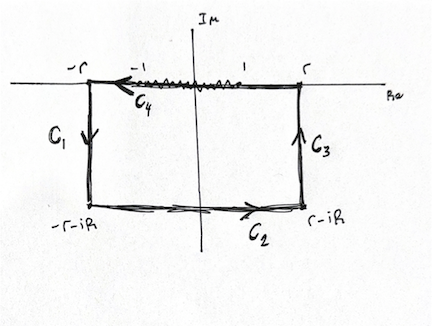
\includegraphics{five-part-one-contour}
	\caption{
		As noted in the main discussion, the closed contour $C$ is broken down into the 4 sides of the rectangular are to be denoted $C_1$ through $C_4$.
	}\label{fig:f1}
\end{figure}
See Figure \ref{fig:f1} for a cartoon of these contours.
\\

Notice the contour $C_4$ traverses along the branch cut from $[-1, 1]$ on the real axis.
We need to account for this by creating a sequence of contours which converge to the actual contours we want to evaluate the integral over. \\
\begin{figure}[h]
	\centering
	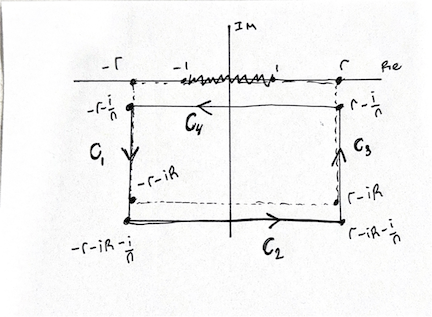
\includegraphics{five-part-one-sequence}
	\caption{
		This diagram represents the original closed contour $C$ being entirely shifted down by $\I / n$.
		This helps us construct the sequence of contours which converge to the original contour we really want to evaluate.
	}\label{fig:f2}
\end{figure}

\noindent
As seen in Figure \ref{fig:f2}, we will be shifting our whole region $\Sigma$ (and thus our contour $C = \partial \Sigma$) down away from the real axis and the branch cut.
We will then construct a sequence of contours which converge to the contour we want.
This can be done by constructing parameterizations of our contours $C_j$ such that 
\begin{align*}
	z_{j_n}(t) \overset{n \to \infty}{\longrightarrow} z_j(t)  \:\: \text{ and} \:\:
	z_{j_n}'(t) \overset{n \to \infty}{\longrightarrow} z'_j(t), \:\: \text{both uniformly on } [a,b].
\end{align*}
Where $z_j(t)$ is a parameterization of $C_j$, $z_{j_n}(t)$ is a sequence of functions which converge uniformly to $z_j(t)$, similarly for the derivative of this parameterization, and $a$ and $b$ are the points such that $z_j(a) = z_0$ and $z_j(b) = z_{\star}$ the initial and terminating points on the contour $C_j$. \\

\noindent
Now let's discuss the specific parameterizations of these contours and their uniformly convergent sequences of functions.
\begin{align*}
&z_{1_n}(t) = -r - \I/n -\I R t \quad t \in [0, 1]& &z_1(t) = -r -\I R t \quad t \in [0, 1]& \\
&z_{2_n}(t) = -r - \I R - \I/n + 2rt \quad t \in [0, 1]& &z_2(t) = -r - \I R + 2rt \quad t \in [0, 1]& \\
&z_{3_n}(t) = r - \I/n -\I R + \I R t \quad t \in [0, 1]& &z_3(t) = r -\I R + \I R t \quad t \in [0, 1]& \\
&z_{4_n}(t) = r - \I/n - 2rt \quad t \in [0, 1]& &z_4(t) = r - 2rt \quad t \in [0, 1].&
\end{align*}
I will demonstrate how a few of these are indeed uniformly convergent. I argue that the other cases I will not discuss can be shown similarly.
Let $\epsilon > 0$ and choose $N = \ceil{\frac 1 \epsilon}$ such that whenever $n > N$ we have the following
\begin{align*}
\left| z_{1_n}(t) - z_1(t) \right|
	&= \left| -r - \I/n -\I R t - \left(-r -\I R t\right) \right| \\
	&= \left| \cancel{-r} - \I/n - \cancel{\I R t} + \cancel{r} + \cancel{\I R t} \right| \\
	&= \left| - \frac \I n \right| \\
	&< \left| - \frac \I {\frac 1 \epsilon} \right| \\
	&= \left| - \I \epsilon \right| \\
	&= \epsilon.
\end{align*}
Therefore, $\left| z_{1_n}(t) - z_1(t) \right| < \epsilon$ and $z_{1_n}(t)$ converges uniformly to $z_1(t)$ since for all $n > N$ our criteria holds and the $N$ does not depend on the value of $t$.
This is the parameterization of the left hand side of our rectangular contour.
Let's now verify this for perhaps the more crucial of our parameterized sequences of contours which is the top of the rectangular contour, the one which we hope traverses along the branch cut in the limit.
Let $\epsilon > 0$ and choose $N = \ceil{\frac 1 \epsilon}$ such that whenever $n > N$ then
\begin{align*}
\left| z_{4_n}(t) - z_4(t) \right|
	&= \left| r - \I/n - 2rt - (r - 2rt) \right| \\
	&= \left| \cancel{r} - \I/n - \cancel{2rt} - \cancel{r} + \cancel{2rt} \right| \\
	&= \left| - \frac \I n \right| \\
	&< \left| - \frac \I {\frac 1 \epsilon} \right| \\
	&= \left| - \I \epsilon \right| \\
	&= \epsilon.
\end{align*}
Therefore, $\left| z_{4_n}(t) - z_4(t) \right| < \epsilon$ and $z_{4_n}(t)$ converges uniformly to $z_4(t)$ since for all $n > N$ our criteria holds and the $N$ does not depend on the value of $t$.
Similarly, $z_{3_n}(t)$ and $z_{4_n}(t)$ converge uniformly to $z_3(t)$ and $z_4(t)$, respectively.
And their derivatives give us,
\begin{align*}
&z_{1_n}^\prime(t) = -\I R \quad t \in [0, 1]& &z_1^\prime(t) = -\I R \quad t \in [0, 1]& \\
&z_{2_n}^\prime(t) = 2r \quad t \in [0, 1]& &z_2^\prime(t) = 2r \quad t \in [0, 1]& \\
&z_{3_n}^\prime(t) = \I R \quad t \in [0, 1]& &z_3^\prime(t) = \I R \quad t \in [0, 1]& \\
&z_{4_n}^\prime(t) = - 2r \quad t \in [0, 1]& &z_4^\prime(t) = - 2r \quad t \in [0, 1].&
\end{align*}
Since, for each $z_{j_n}(t)$ and $z_{j_n}^\prime(t)$ we have that
\begin{align*}
	z_{j_n}(t) \overset{n \to \infty}{\longrightarrow} z_j(t)  \:\: \text{ and} \:\:
	z_{j_n}'(t) \overset{n \to \infty}{\longrightarrow} z'_j(t), \:\: \text{both uniformly on } [0,1].
\end{align*}
Therefore by Lemma 1 established in problem 4, we can say
\begin{align*}
\oint_{C_{j_n}}h(z)\D z \overset{n \to \infty}{\longrightarrow} \oint_{C_j}h(z)\D z
\end{align*}
for each $C_j$.
By our carful decomposition of the original contour $C$ and the parameterizations of each component of $C$, we can say 
$$\oint_{C_n} h(z) \D z = \sum_{j = 1}^{4} \oint_{C_{j_n}}h(z) \D z \rightarrow \sum_{j = 1}^{4} \oint_{C_j}h(z) \D z = \oint_{C}h(z)\D z.$$
Hence,
$$\oint_{C_n}h(z)\D z \overset{n \to \infty}{\longrightarrow} \oint_{C}h(z)\D z.$$
Since $h(z)$ is analytic in the region containing our sequence of simple closed contours $C_n$ then by Cauchy's Theorem
$$
\oint_{C_n}h(z)\D z = 0.
$$
Therefore, we must also have
$$\oint_{C}h(z)\D z = 0$$
since the sequence $\oint_{C_n}h(z)\D z$ (which turns out is a sequence of zeros), converges to $\oint_{C}h(z)\D z$. \\
\qed \\

  \item Show that if $f(z)$ is analytic in a region that contains $\Sigma$
    \begin{align*}
        \oint_C \frac{f(z) \D z}{\sqrt{z-1} \sqrt{z+1}}= 0.
      \end{align*}
\textit{Solution:} \\
There are a few cases to address here.
First, of all if $r < 1$ then our contour $C$ does not intersect any points where $h(z)$ (same notation as in part 1) is undefined or blows up.
In this case evaluating this integral is the same as the part 1.
I also claim that the case when $r=1$ is the same as part 1 as well.
Since we are still not strictly integrating across either problematic point but they are instead at the bounds of integration for the contour integrals we have no issues and again can refer to part 1 in this case.
The more interesting case is when $r > 1$.
Let's address this case thoroughly and carefully. \\

\noindent
Let's use the same parameterizations of each side of the rectangular contour except for the $C_4$ section, we will define the contour $C_4$ in a new way.
I am defining $\widehat C$ to be the top of the rectangle from part 1.
This time we cut out two lower half plane semicircles from the contour $C_4$ to make $\widehat C$.
Now let's break down $\widehat C$ into 5 separate contours $\widehat C_k$ where $k \in \{1, 2, ..., 5\}$.
We define these contours as follows
\begin{align*}
&\widehat C_1: \: \text{a horizontal line in the complex plane from } z_0=r \: \text{ to }  z_{\star}=1 + \epsilon \\
&\widehat C_2: \: \text{semicircle in the lower half plane centered at $z=1$ with radius $\epsilon$}, z_0=1 + \epsilon \: \text{ to }  z_{\star}=1 - \epsilon \\
&\widehat C_3: \: \text{a horizontal line in the complex plane from } z_0=1 - \epsilon \: \text{ to }  z_{\star}=-1 + \epsilon \\
&\widehat C_4: \: \text{semicircle in the lower half plane centered at $z=-1$ with radius $\epsilon$},  z_0=-1 + \epsilon \: \text{ to }  z_{\star}=-1 - \epsilon \\
&\widehat C_5: \: \text{a horizontal line in the complex plane from } z_0=-1 - \epsilon \: \text{ to }  z_{\star}=-r.
\end{align*}
We now parameterize things with a sequence of contours to help us apply results from lemma 1 (let's denote these with hats to mean $\hat z$ are values of $z$ along $\widehat C$)
\begin{align*}
&\hat z_{2_n}(t) = \epsilon \E^{\I \theta} + 1 - \frac \I n \quad \theta \in [0, -\pi]&
	&\hat z_2(t) = \epsilon \E^{\I \theta} + 1 \quad \theta \in [0, -\pi]& \\
&\hat z_{4_n}(t) = \epsilon \E^{\I \theta} - 1 - \frac \I n \quad \theta \in [0, -\pi]&
	&\hat z_4(t) = \epsilon \E^{\I \theta} - 1 \quad \theta \in [0, -\pi]& \\
&\hat z_{1_n}(t) = r + (1 + \epsilon - r)t - \frac \I n \quad t \in [0, 1]&
	&\hat z_1(t) = r + (1 + \epsilon - r)t \quad t \in [0, 1]& \\
&\hat z_{3_n}(t) = 1 - \epsilon - 2(1 - \epsilon)t - \frac \I n \quad t \in [0, 1]&
	&\hat z_3(t) = 1 - \epsilon - 2(1 - \epsilon)t \quad t \in [0, 1]& \\
&\hat z_{5_n}(t) = - 1 - \epsilon + (- r + 1 + \epsilon)t - \frac \I n\quad t \in [0, 1]&
	&\hat z_5(t) = - 1 - \epsilon + (- r + 1 + \epsilon)t \quad t \in [0, 1].&
\end{align*}
See Figure \ref{fig:f3} for a helpful cartoon to visualize this new contour path.
I will demonstrate how a few of these are indeed uniformly convergent.
I argue that the other cases I will not discuss can be shown similarly.
Let $\epsilon > 0$ and choose $N = \ceil{\frac 1 \epsilon}$ such that whenever $n > N$ we have the following
\begin{align*}
\left| \hat z_{1_n}(t) - \hat z_1(t) \right|
	&= \left| r + (1 + \epsilon - r)t - \frac \I n - \left(r + (1 + \epsilon - r)t\right) \right| \\
	&= \left| \cancel{r + (1 + \epsilon - r)t} - \frac \I n - \cancel {\left(r + (1 + \epsilon - r)t\right)} \right| \\
	&= \left| - \frac \I n \right| \\
	&< \left| - \frac \I {\frac 1 \epsilon} \right| \\
	&= \left| - \I \epsilon \right| \\
	&= \epsilon.
\end{align*}
Once again, let $\epsilon > 0$ and choose $N = \ceil{\frac 1 \epsilon}$ such that whenever $n > N$ we have the following
\begin{align*}
\left| \hat z_{2_n}(t) - \hat z_2(t) \right|
	&= \left| \epsilon \E^{\I \theta} + 1 - \frac \I n - \left(\epsilon \E^{\I \theta} + 1\right) \right| \\
	&= \left| \cancel{\epsilon \E^{\I \theta} + 1} - \frac \I n - \cancel{\left(\epsilon \E^{\I \theta} + 1\right)} \right| \\
	&= \left| - \frac \I n \right| \\
	&< \left| - \frac \I {\frac 1 \epsilon} \right| \\
	&= \left| - \I \epsilon \right| \\
	&= \epsilon.
\end{align*}
\begin{figure}[h]
	\centering
	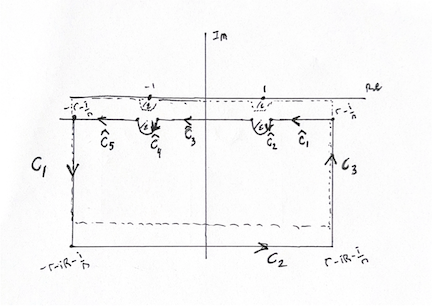
\includegraphics{five-part-two-sequence}
	\caption{
		This cartoon represents the new ``ticket-stub" closed contour $C$ being entirely shifted down by $\I / n$.
		The semicircles have a fixed radius $0< \epsilon < 1$.
		See the careful parameterizations of the contours $\widehat C_1$ through $\widehat C_5$.
	}\label{fig:f3}
\end{figure}
And their derivatives give us,
\begin{align*}
&\hat z_{2_n}^\prime(t) = \epsilon \I \E^{\I \theta} \quad \theta \in [0, -\pi]&
	&\hat z_2^\prime(t) = \epsilon \I \E^{\I \theta} \quad \theta \in [0, -\pi]& \\
&\hat z_{4_n}^\prime(t) = \epsilon \I \E^{\I \theta} \quad \theta \in [0, -\pi]&
	&\hat z_4^\prime(t) = \epsilon \I \E^{\I \theta} \quad \theta \in [0, -\pi]& \\
&\hat z_{1_n}^\prime(t) = 1 + \epsilon - r \quad t \in [0, 1]&
	&\hat z_1^\prime(t) = 1 + \epsilon - r \quad t \in [0, 1]& \\
&\hat z_{3_n}^\prime(t) = - 2(1 - \epsilon) \quad t \in [0, 1]&
	&\hat z_3^\prime(t) = - 2(1 - \epsilon) \quad t \in [0, 1]& \\
&\hat z_{5_n}^\prime(t) = - r + 1 + \epsilon \quad t \in [0, 1]&
	&\hat z_5^\prime(t) = - r + 1 + \epsilon \quad t \in [0, 1].&
\end{align*}
Now that we have these continuous sequences which converge uniformly I site lemma 1 to conclude that we have
$$
\oint_{C_{j_n}}h(z)\D z \overset{n\rightarrow \infty}{\longrightarrow} \oint_{C_j} h(z)\D z \quad \text{for each} \: j \in \{1, 2, 3\}
$$
and
$$
\oint_{\widehat C_{j_n}}h(z)\D z \overset{n\rightarrow \infty}{\longrightarrow} \oint_{\widehat C_j} h(z)\D z \quad \text{for each} \: j \in \{1, 2, 3, 4, 5\}.
$$
We have shown how we can use lemma 1 to create a sequence of ``ticket-stub" shaped contours which converge to the ``ticket-stub" shaped contour which is on the real axis and partially traverses along the branch cut.
Now we want to shrink these open semicircles in the lower half plane by letting the radius $\epsilon$ go to 0.
See the cartoon depiction of this in Figure \ref{fig:f4} for more details.
\begin{figure}[h]
	\centering
	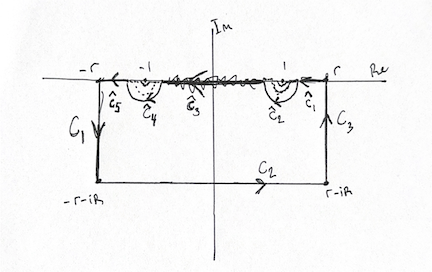
\includegraphics{five-part-two-contour}
	\caption{
		This cartoon represents the new ``ticket-stub" closed contour $C$ now that it's on the real axis.
		We are now shrinking the radii of the semicircles by setting $\epsilon = \frac 1 k$.
		See the careful parameterizations of the contours $\widetilde C_1$ through $\widetilde C_5$ for how this shrinking works.
	}\label{fig:f4}
\end{figure}
If we let $\epsilon = 1/k$ and let $k\rightarrow \infty$ then we will end up with the the original $C_4$.
We denote this final collection of contours and parameterizations with the tilde symbol as follows $
\widetilde C_j$ and $\tilde z_j(t)$.
Then we have the following contours that makeup the contour $C_4$
\begin{align*}
&\widetilde C_1: \: \text{a horizontal line in the complex plane from } z_0=r \: \text{ to }  z_{\star}=1 \\
&\widetilde C_2: \: \text{a single point}, z_0=z_\star=1 \\
&\widetilde C_3: \: \text{a horizontal line in the complex plane from } z_0=1 \: \text{ to }  z_{\star}=-1 \\
&\widetilde C_4: \: \text{a single point}, z_0=z_\star=-1 \\
&\widetilde C_5: \: \text{a horizontal line in the complex plane from } z_0=-1 \: \text{ to }  z_{\star}=-r.
\end{align*}
Furthermore, we have the following sequences of parameterizations
\begin{align*}
&\hat z_{2_k}(t) = (1/k) \E^{\I \theta} + 1\quad \theta \in [0, -\pi]&
	&\hat z_2(t) = 1 \quad \theta \in [0, -\pi]& \\
&\hat z_{4_k}(t) = (1/k) \E^{\I \theta} - 1 \quad \theta \in [0, -\pi]&
	&\hat z_4(t) = - 1 \quad \theta \in [0, -\pi]& \\
&\hat z_{1_k}(t) = r + (1 + (1/k) - r)t  \quad t \in [0, 1]&
	&\hat z_1(t) = r + (1 - r)t \quad t \in [0, 1]& \\
&\hat z_{3_k}(t) = 1 - (1/k) - 2(1 - (1/k))t  \quad t \in [0, 1]&
	&\hat z_3(t) = 1 - 2t \quad t \in [0, 1]& \\
&\hat z_{5_k}(t) = - 1 - (1/k) + (- r + 1 + (1/k))t \quad t \in [0, 1]&
	&\hat z_5(t) = - 1 + (- r + 1)t \quad t \in [0, 1].&
\end{align*}
And the derivatives
\begin{align*}
&\hat z_{2_k}(t) = (1/k)\I \E^{\I \theta} \quad \theta \in [0, -\pi]&
	&\hat z_2(t) = 0 \quad \theta \in [0, -\pi]& \\
&\hat z_{4_k}(t) = (1/k)\I \E^{\I \theta} \quad \theta \in [0, -\pi]&
	&\hat z_4(t) = 0 \quad \theta \in [0, -\pi]& \\
&\hat z_{1_k}(t) = 1 + (1/k) - r  \quad t \in [0, 1]&
	&\hat z_1(t) = 1 - r \quad t \in [0, 1]& \\
&\hat z_{3_k}(t) = - 2(1 - (1/k))  \quad t \in [0, 1]&
	&\hat z_3(t) = - 2 \quad t \in [0, 1]& \\
&\hat z_{5_k}(t) = - r + 1 + (1/k) \quad t \in [0, 1]&
	&\hat z_5(t) = - r + 1 \quad t \in [0, 1].&
\end{align*}
\\

\noindent
Additionally in order to use lemma 1 again, we need to have continuity of $h(z)$ on the closure of our open set
$$\Omega = \{z \: : \: -R < \Im(z) < 0 \} \cap \{z \: : \: -r < \Re(z) < r \}.$$
Since $\overline \Omega$ includes $-1$ and $1$, the points that $h(z)$ blows up or is not defined, we need to do some more work before applying lemma 1
We need to establish continuity at these points, let's define an extension of h(z) such that
\begin{align*}
h(-1) &= \frac 1 {2\pi \I}\oint_C \frac {h(\xi)}{\xi + 1} \D \xi \\
h(1) &= \frac 1 {2\pi \I}\oint_C \frac {h(\xi)}{\xi - 1} \D \xi.
\end{align*}
Using this let's establish continuity at these points of concern.
Notice
\begin{align*}
\lim_{z \rightarrow -1} \left| h(-1) - h(z) \right|
	&= \lim_{z \rightarrow -1} \left| \frac 1 {2\pi \I} \oint_C \frac {h(\xi)}{\xi + 1} \D \xi - \frac 1 {2\pi \I}\oint_C \frac {h(\xi)}{\xi - z} \D \xi \right| \\
	&= \lim_{z \rightarrow -1} \left| \frac 1 {2\pi \I} \oint_C \frac {h(\xi)}{\xi + 1} -  \frac {h(\xi)}{\xi - z} \D \xi \right| \\
	&= \lim_{z \rightarrow -1} \left| \frac 1 {2\pi \I} \oint_C \frac {h(\xi)(\xi - z) - h(\xi)(\xi + 1)}{(\xi - z)(\xi + 1)} \D \xi \right| \\
	&= \lim_{z \rightarrow -1} \left| \frac 1 {2\pi \I} \oint_C \frac {\cancel{h(\xi)\xi} - h(\xi)z - \cancel{h(\xi)\xi} - h(\xi)}{(\xi - z)(\xi + 1)} \D \xi \right| \\
	&= \lim_{z \rightarrow -1} \left| \frac 1 {2\pi \I} \oint_C \frac {h(\xi)(- 1 - z)}{(\xi - z)(\xi + 1)} \D \xi \right| \\
	&= \lim_{z \rightarrow -1} \left| \frac {-1 - z} {2\pi \I} \oint_C \frac {h(\xi)}{(\xi - z)(\xi + 1)} \D \xi \right| \\
	&= \lim_{z \rightarrow -1} \left| \frac {-1 - z} {2\pi \I} \right| \left|\oint_C \frac {h(\xi)}{(\xi - z)(\xi + 1)} \D \xi \right| \\
	&= 0.
\end{align*}
Since $(-1-z)\overset{z \to -1}{\longrightarrow} 0$ and the value of the integral, namely it's denominator, will not go to 0.
Therefore $h(z)$ is continuous at the point $z = -1$.
Similarly,
\begin{align*}
\lim_{z \rightarrow 1} \left| h(1) - h(z) \right|
	&= \lim_{z \rightarrow 1} \left| \frac 1 {2\pi \I} \oint_C \frac {h(\xi)}{\xi - 1} \D \xi - \frac 1 {2\pi \I}\oint_C \frac {h(\xi)}{\xi - z} \D \xi \right| \\
	&= \lim_{z \rightarrow 1} \left| \frac 1 {2\pi \I} \oint_C \frac {h(\xi)}{\xi - 1} -  \frac {h(\xi)}{\xi - z} \D \xi \right| \\
	&= \lim_{z \rightarrow 1} \left| \frac 1 {2\pi \I} \oint_C \frac {h(\xi)(\xi - z) - h(\xi)(\xi - 1)}{(\xi - z)(\xi - 1)} \D \xi \right| \\
	&= \lim_{z \rightarrow 1} \left| \frac 1 {2\pi \I} \oint_C \frac {\cancel{h(\xi)\xi} - h(\xi)z - \cancel{h(\xi)\xi} + h(\xi)}{(\xi - z)(\xi - 1)} \D \xi \right| \\
	&= \lim_{z \rightarrow 1} \left| \frac 1 {2\pi \I} \oint_C \frac {h(\xi)(1 - z)}{(\xi - z)(\xi - 1)} \D \xi \right| \\
	&= \lim_{z \rightarrow 1} \left| \frac {1 - z} {2\pi \I} \oint_C \frac {h(\xi)}{(\xi - z)(\xi - 1)} \D \xi \right| \\
	&= \lim_{z \rightarrow 1} \left| \frac {1 - z} {2\pi \I} \right| \left|\oint_C \frac {h(\xi)}{(\xi - z)(\xi - 1)} \D \xi \right| \\
	&= 0.
\end{align*}
Since $(1-z)\overset{z \to 1}{\longrightarrow} 0$ and the value of the integral, namely it's denominator, will not go to 0.
Therefore $h(z)$ is continuous at the point $z = 1$.
Now that we have $h(z)$ is continuous on the closure of our open set $\Omega$, we can site lemma 1 to conclude that 
$$
\oint_{\widetilde C_{j_k}} h(z) \D z \overset{n\rightarrow \infty}{\longrightarrow} \oint_{\widetilde C_j} h(z) \D z \quad \text{for each } j \in \{1, 2, ..., 5\}.
$$
Notice, the way we defined the $\widetilde C_j$'s we end up with 
$$
\sum_{j=1}^5 \oint_{\widetilde C_j} h(z) \D z = \oint_{C_4} h(z) \D z.
$$
Therefore, once again we have $h(z)$ is analytic in the region containing our sequence of simple closed contours $C_n$ then by Cauchy's Theorem
$$
\oint_{C_n}h(z)\D z = 0.
$$
Therefore, we must also have
$$\oint_{C}h(z)\D z = 0$$
since the sequence $\oint_{C_n}h(z)\D z$ (which turns out is a sequence of zeros), converges to $\oint_{C}h(z)\D z$.


\end{itemize}
\newpage

\item From A\&F: 3.1.1 b,d \\
In the following we are given sequences.
Discuss their limits and whether the convergence is uniform, in the region $\alpha \leq |z| \leq \beta$, for finite $\alpha, \beta > 0$. \\
b) $$ \bigg\{ \frac 1 {z^n} \bigg\}_{n=1}^{\infty} $$
\textit{Solution:}\\
Let $f_n(z) = \frac 1 {z^n}$, for $n \in \mathbb N$. Then we notice
$$
f_n(z) \overset{n \to \infty}{\longrightarrow} \begin{cases}
0, \quad \quad \quad \quad \quad \: \: \text{if}\: |z| > 1 \\
1, \quad \quad \quad \quad \quad \: \: \text{if}\: z = 1 \\
\text{diverges}, \quad \quad \: \: \text{if}\: |z| = 1, z \neq 1 \\
\text{diverges to } \infty, \text{if}\: |z| < 1.
\end{cases}
$$
I will now demonstrate that this sequence is uniformly convergent when $|z| < 1$, which in terms of $\alpha$ and $\beta$ is any of the cases where
$$1 <\alpha \leq |z| \leq \beta < \infty.$$
Taking the limit of this function directly, we see
\begin{align*}
\lim_{n\rightarrow \infty} \left| f_n(z) - 0 \right|
	&= \lim_{n\rightarrow \infty} \left| f_n(z)\right| \\
	&= \lim_{n\rightarrow \infty} \left| \frac 1 {z^n} \right| \\
	&= \lim_{n\rightarrow \infty} \frac 1 {\left| {z^n} \right|} \\
	&= 0.
\end{align*}
This is because $|z^n|$ is a number with modulus greater than 1 being raised to a positive power, so it blows up.
As the denominator blows up the whole expression goes to 0.
Therefore, $f_n(z)$ converges uniformly to $0$ when we have these constraints on $|z|$.
Furthermore, the case where $z = 1$, $f_n(z)$ is vacuously uniformly convergent. It does not depend on the value of $z$ because in this scenario $z$ is constantly $1$ so we are asking ourselves what is the convergence of
$$\frac 1 {1^n}.$$
We know $1$ raised to any power is just $1$. So as $n \rightarrow \infty$, we just get
$$ \frac 1 {1^n} \overset{n \to \infty}{\longrightarrow} 1.$$
However, generally, the convergence of this sequence $f_n(z)$ cannot be uniform, since the limit is not continuous. \\
\qed \\

\newpage

\noindent
d) $$ \bigg\{ \frac 1 {1 + (nz)^2} \bigg\}_{n=1}^{\infty} $$
\textit{Solution:}\\
Let $f_n(z) = \frac 1 {1 + (nz)^2}$, for $n \in \mathbb N$. Then we notice
$$
f_n(z) \overset{n \to \infty}{\longrightarrow} \begin{cases}
1, \: \: \text{if}\: |z| = 0 \\
0, \: \: \text{if}\: |z| > 0.
\end{cases}
$$
However, since we have $|z| \geq \alpha > 0$ we know $|z| \neq 0$ and thus
$$
f_n(z) \overset{n \to \infty}{\longrightarrow} 0 \quad \text{uniformly}.
$$
This result is independent of the choice of upper bound $\beta$.
More formally, I will show it using the limit.
Notice,
\begin{align*}
\lim_{n \rightarrow \infty} \left| f_n(z) - f(z) \right|
	&= \lim_{n \rightarrow \infty} \left| \frac 1 {1 + (nz)^2} - 0 \right| \\
	&= \lim_{n \rightarrow \infty} \left| \frac 1 {1 + (nz)^2}\right| \\
	&= \lim_{n \rightarrow \infty} \frac 1 {|1 + n^2z^2|} \\
	&= \lim_{n \rightarrow \infty} \frac 1 {|1 + n^2(x + iy)^2|} \\
	&= \lim_{n \rightarrow \infty} \frac 1 {|1 + n^2(x^2 + 2\I x y - y^2) |} \\
	&= \lim_{n \rightarrow \infty} \frac 1 {\sqrt{(1 + n^2x^2 - n^2y^2)^2 + (n^22 x y)^2 }} \\
	&= \lim_{n \rightarrow \infty} \frac 1 {\sqrt{(1 + n^2(x - y)(x + y))^2 + n^4 4 x^2 y^2 }} \\
	&= \lim_{n \rightarrow \infty} \frac 1 {\sqrt{(1 + 2n^2(x - y)(x + y) + n^4(x - y)^2(x + y)^2 + n^4 4 x^2 y^2 }}
\end{align*}
We want to show that this limit is 0. this will help with the uniform convergence arguments to be made.
\qed
\newpage

\item From A\&F: 3.1.2 b,d \\
For each sequence in problem 6 (book problem 1), what can be said if \\
\textit{Solution:} \\
(b) Now let's begin by reconsidering the sequence from the previous problem, part (b).
Let $f_n(z) = \frac 1 {z^n}$, for $n \in \mathbb N$. Then we notice
$$
f_n(z) \overset{n \to \infty}{\longrightarrow} \begin{cases}
0, \: \: \text{if}\: |z| > 1 \\
1, \: \: \text{if}\: |z| = 1 \\
\infty, \text{if}\: |z| < 1.
\end{cases}
$$
Let's now consider the two cases presented herein. \\

\underline{(a) $\alpha = 0$:} \\
This gives us the following bounds $0 \leq |z| \leq \beta$.
First of all, this now includes the point $z = 0$ for which $f_n(z)$ is not defined.
Second of all, these bounds include all 3 cases for the limit of $f_n(z)$ and is therefore discontinuous.
Hence, our sequence is not uniformly convergent in this case. \\

\underline{(b) $\alpha > 0$ and $\beta = \infty$:} \\
This gives us the following bounds $0 < |z| \leq \infty$.
We are still left with a discontinuous limit of $f_n(z)$ meaning the sequence does not converge uniformly. \\
\qed \\

\noindent
(d) Let $f_n(z) = \frac 1 {1 + (nz)^2}$, for $n \in \mathbb N$. Then we notice
$$
f_n(z) \overset{n \to \infty}{\longrightarrow} \begin{cases}
1, \: \: \text{if}\: |z| = 0 \\
0, \: \: \text{if}\: |z| > 0.
\end{cases}
$$
However, since we have $|z| \geq \alpha > 0$ we know $|z| \neq 0$ and thus
$$
f_n(z) \overset{n \to \infty}{\longrightarrow} 0 \quad \text{uniformly}.
$$
This result is independent of the choice of upper bound $\beta$. \\

\underline{(a) $\alpha = 0$:} \\
This gives us the following bounds $0 \leq |z| \leq \beta$.
Since $|z|$ can be equal to $0$, the limit of $f_n(z)$ includes both cases provided before and is therefore discontinuous.
Therefore, the sequence $f_n(z)$ cannot be uniformly convergent, given these bounds from $\alpha$ and $\beta$. \\

\underline{(b) $\alpha > 0$ and $\beta = \infty$:} \\
This gives us the following bounds $0 < |z| \leq \infty$.
Thus
$$
f_n(z) \overset{n \to \infty}{\longrightarrow} 0 \quad \text{uniformly}.
$$
\qed \\

\newpage
\item From A\&F: 3.1.3
Compute the integrals
$$
\lim_{n \rightarrow \infty} \int_0^1 nz^{n -1}\D z \quad \text{and} \quad \int_0^1 \lim_{n \rightarrow \infty} \left(nz^{n -1} \right) \D z
$$
and show that they are not equal.
Explain why this is not a counter example to Theorem 3.1.1. (A \&F pg. 111) \\
\textit{Solution:} \\
We can easily evaluate the left limit to be
$$
\lim_{n \rightarrow \infty} \int_0^1 nz^{n -1}\D z = \lim_{n \rightarrow \infty} \left. z^n \right|_0^1 = \lim_{n \rightarrow \infty} 1^n - 0^n = \lim_{n \rightarrow \infty} 1 = 1.
$$
However, on the right we have the improper integral (using a limit as we approach the upper bound $1$)
$$
\lim_{\epsilon \rightarrow 0}\int_0^{1-\epsilon} \lim_{n \rightarrow \infty} \left(nz^{n -1} \right) \D z.
$$
These two functions do not converge to the same thing (proof not necessary since other problems are more hefty.)
This is not a counter example of Theorem 3.1.1 since the sequence
$$
\lim_{n \rightarrow \infty} nz^{n - 1} =
\begin{cases}
0, \text{ if } |z| < 1 \\
\infty \text{ if } |z| = 1
\end{cases}
$$
does not converge uniformly. \\
\qed \\
\end{enumerate}

\end{document}

%%% Local Variables:
%%% mode: latex
%%% TeX-master: t
%%% End:
